% !TEX root = ../agglo_clust_review.tex


% \begin{figure}
% \centering
%         \begin{subfigure}[t]{0.46 \linewidth}
%         \centering
%         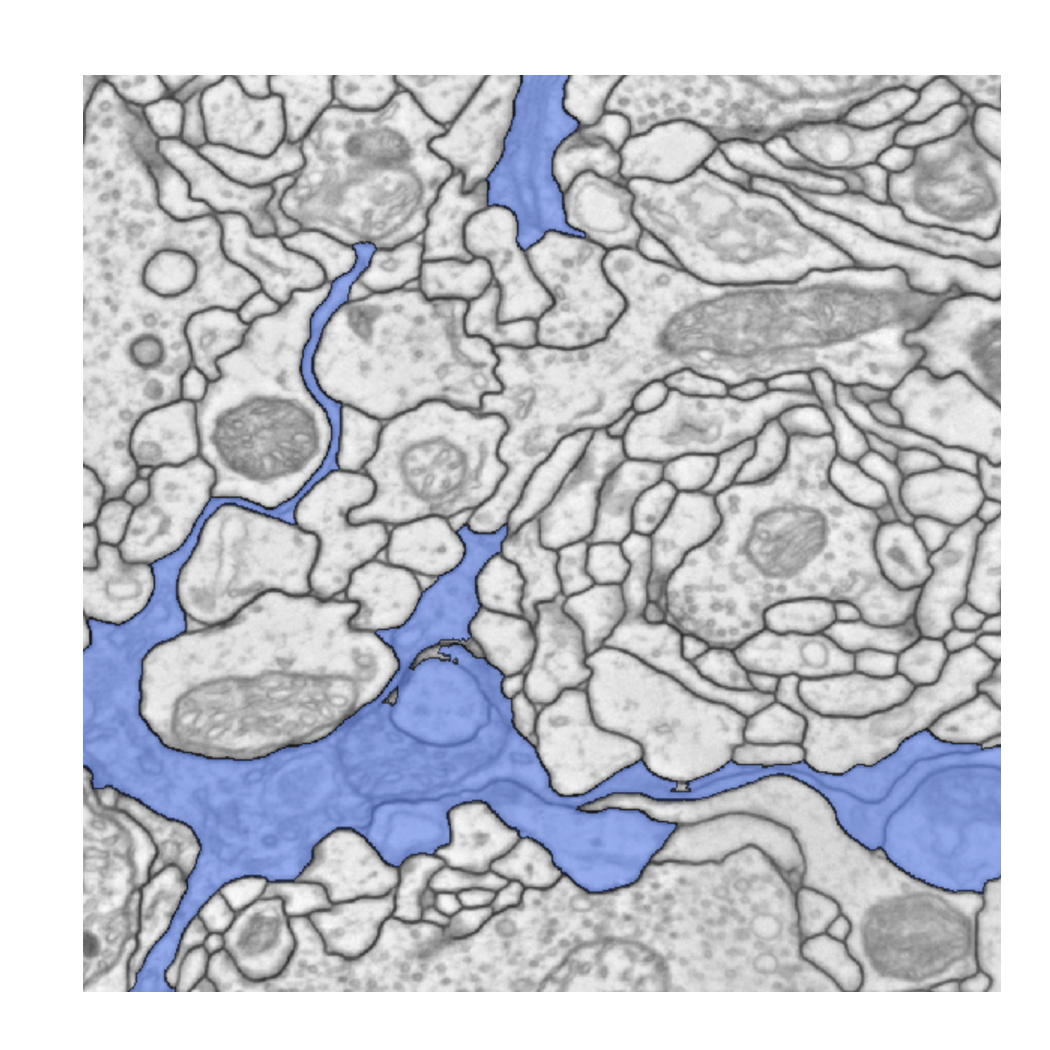
\includegraphics[width=0.98\textwidth]{figs/comparison/sum_F.pdf}
%         % \caption{Thresholding of local boundary maps ~(THRESH)} \label{fig:thresh}
%     \end{subfigure}%
%     \begin{subfigure}[t]{0.46 \linewidth}
%         \centering
%         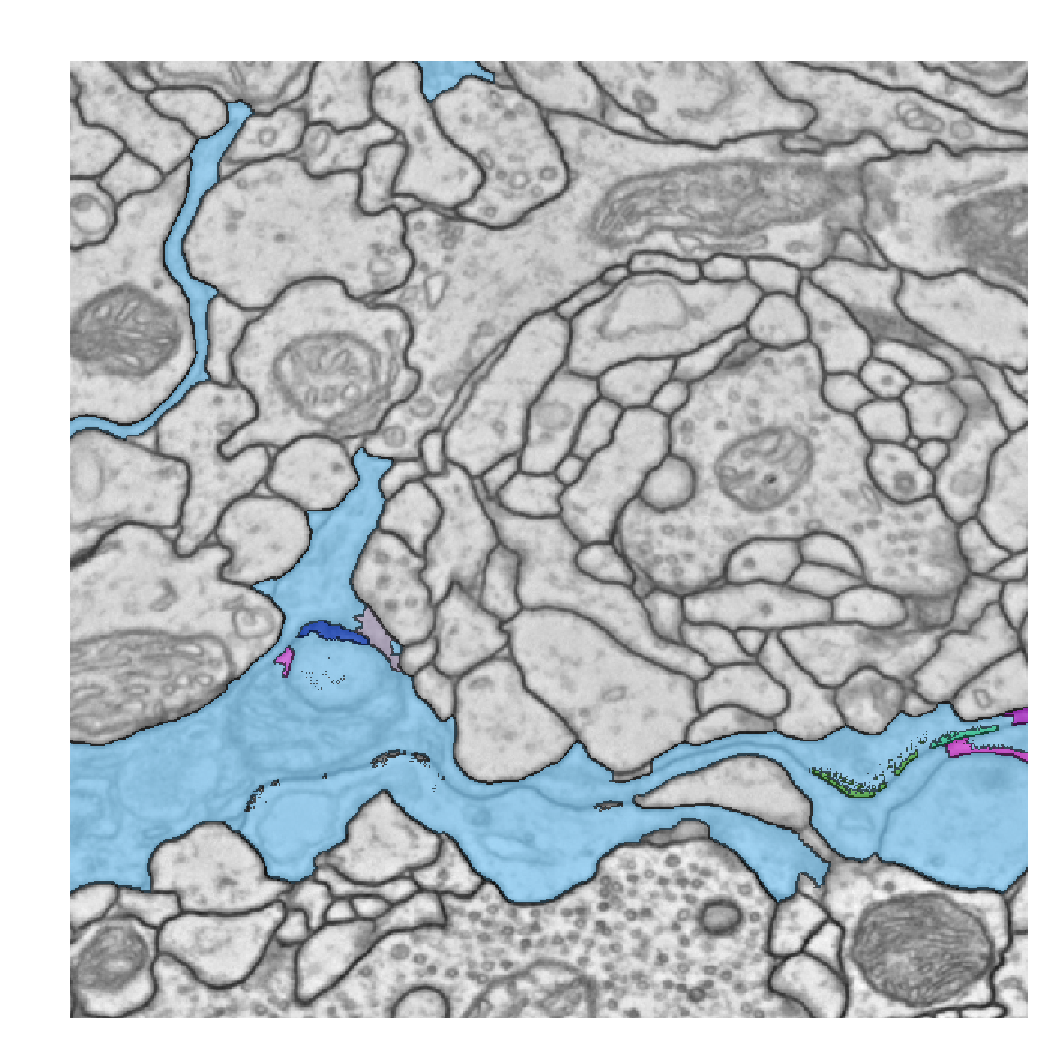
\includegraphics[width=0.98\textwidth]{figs/comparison/sum_T.pdf}
%         % \caption{Watershed, seeded at local minima of the smoothed input map~(WS)} \label{fig:ws}
%     \end{subfigure}\hspace{0.5cm}%

%     % \vspace{0.3cm}
%     \begin{subfigure}[t]{0.92 \linewidth}
%         \centering
%         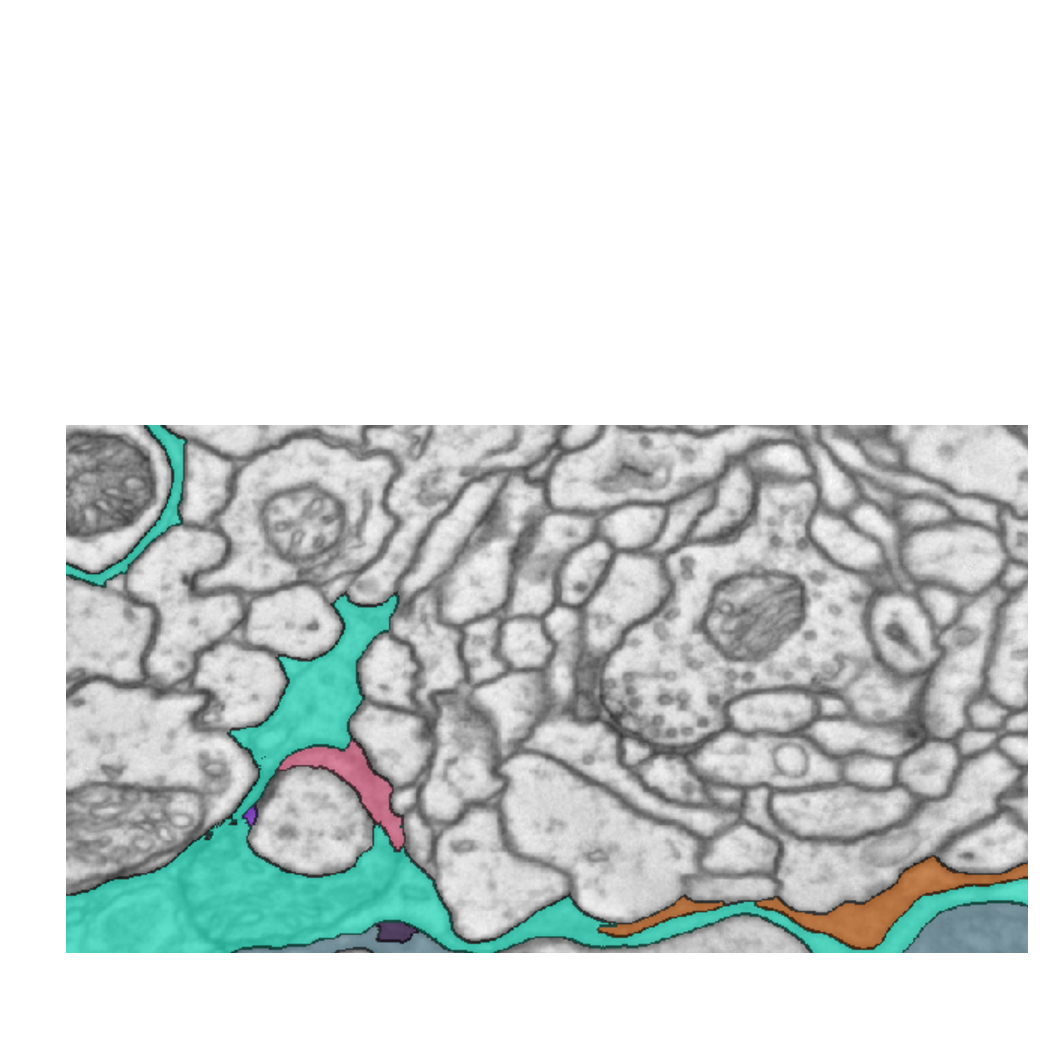
\includegraphics[width=1.\textwidth]{figs/comparison/MWS.pdf}
%         % \caption{Multicut partitioning based segmentation~(MC-FULL)} \label{fig:mc_full}
%     \end{subfigure}\hspace{0.5cm}

%     \begin{subfigure}[t]{0.46 \linewidth}
%         \centering
%         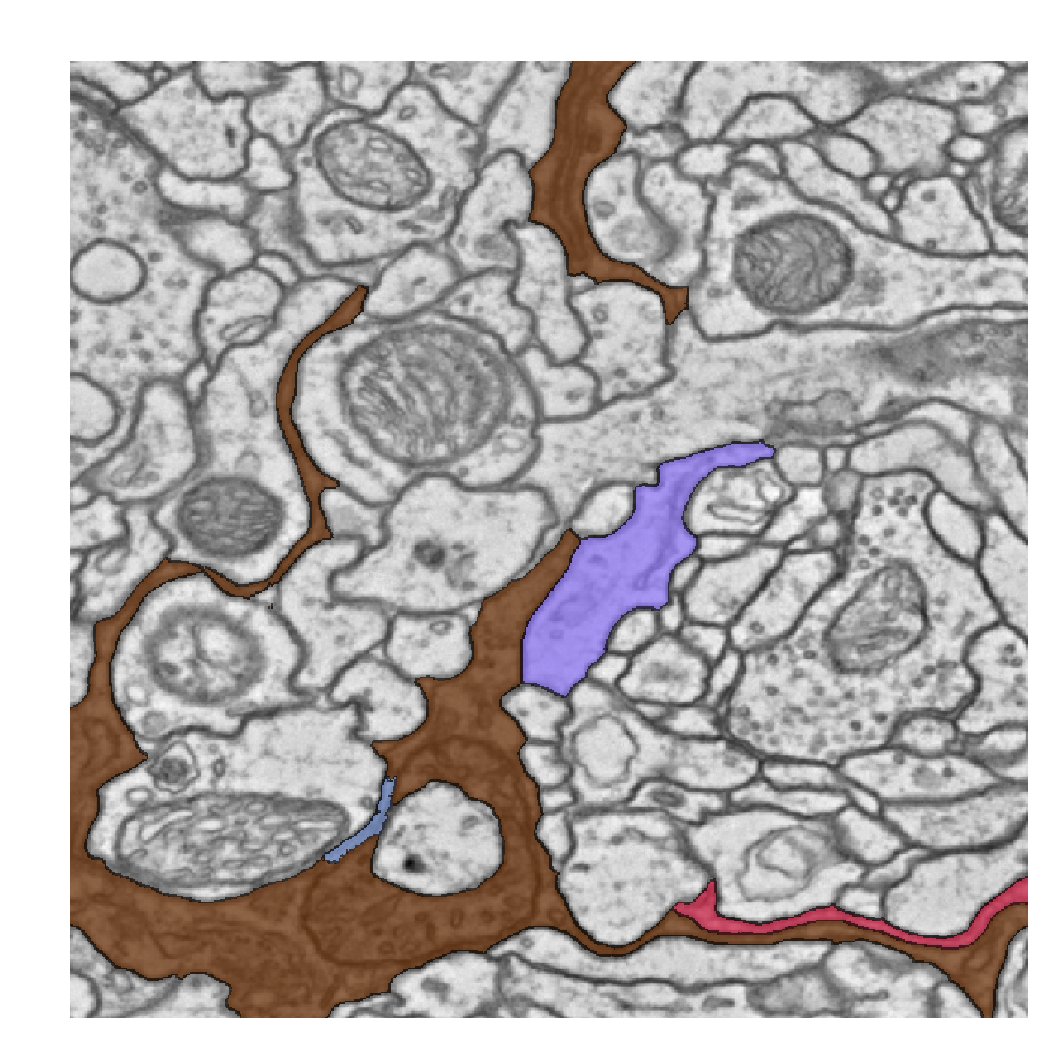
\includegraphics[width=0.98\textwidth]{figs/comparison/mean_F.pdf}
%         % \caption{Thresholding of local boundary maps ~(THRESH)} \label{fig:thresh}
%     \end{subfigure}%
%     \begin{subfigure}[t]{0.46 \linewidth}
%         \centering
%         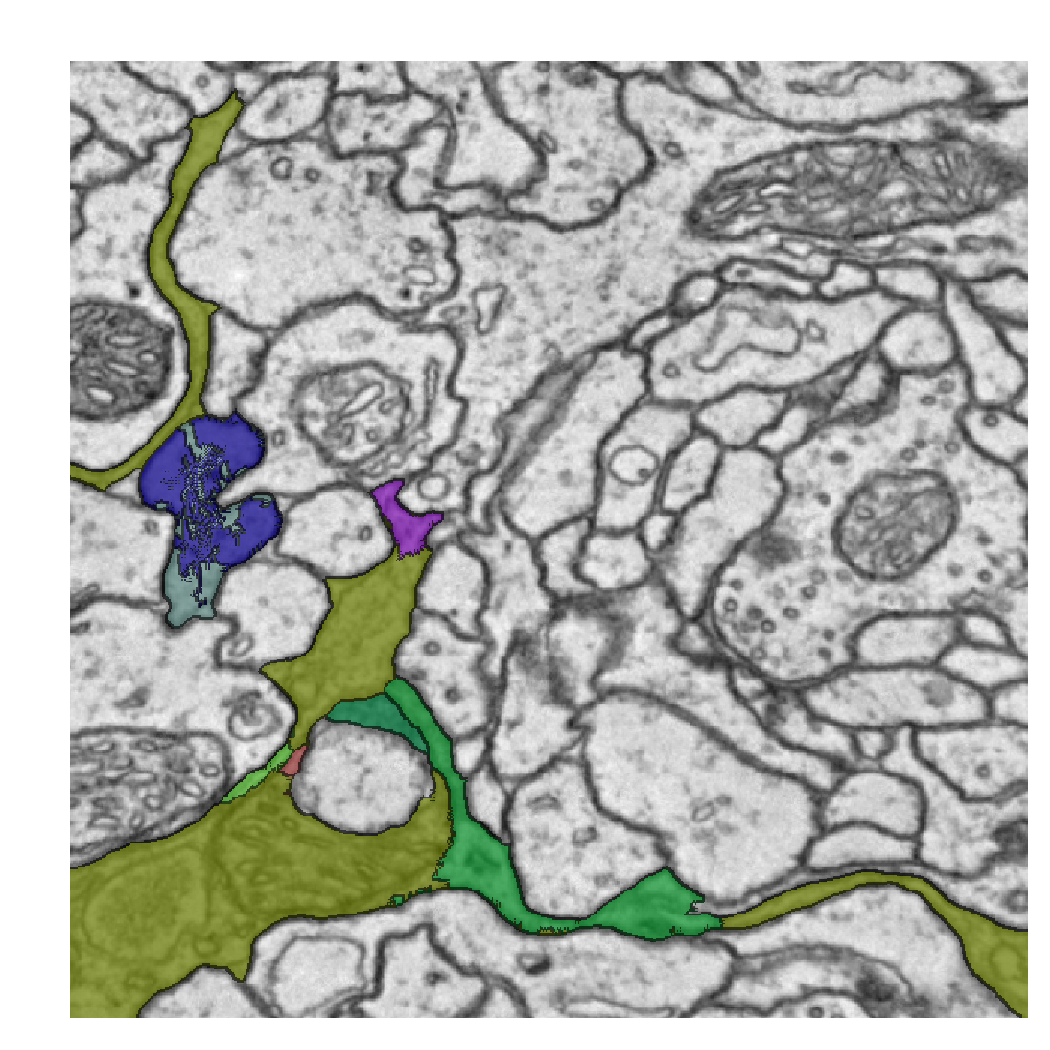
\includegraphics[width=0.98\textwidth]{figs/comparison/mean_T.pdf}
%         % \caption{Watershed, seeded at local minima of the smoothed input map~(WS)} \label{fig:ws}
%     \end{subfigure}\hspace{0.5cm}%

% \begin{subfigure}[t]{0.46 \linewidth}
%         \centering
%         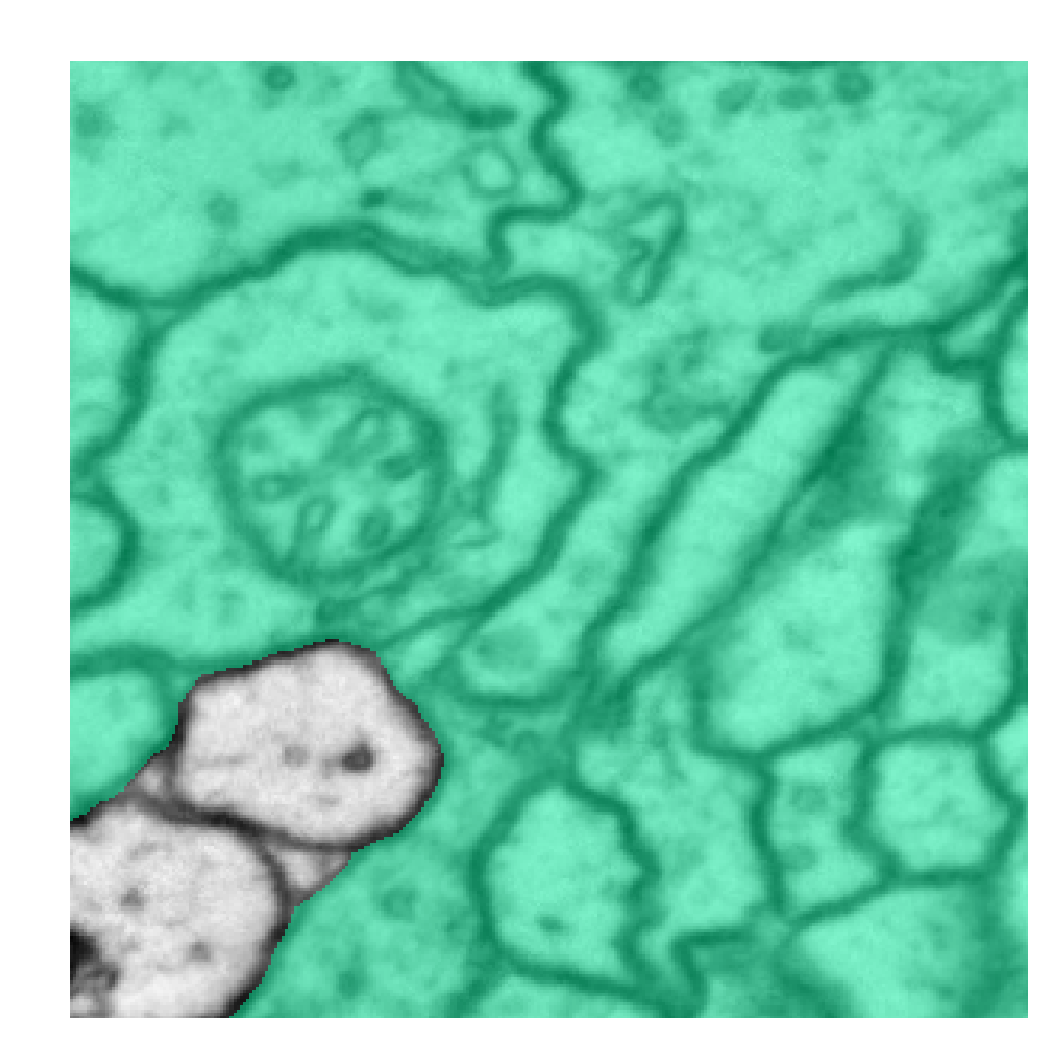
\includegraphics[width=0.98\textwidth]{figs/comparison/max_F.pdf}
%         % \caption{Thresholding of local boundary maps ~(THRESH)} \label{fig:thresh}
%     \end{subfigure}%
%     \begin{subfigure}[t]{0.46 \linewidth}
%         \centering
%         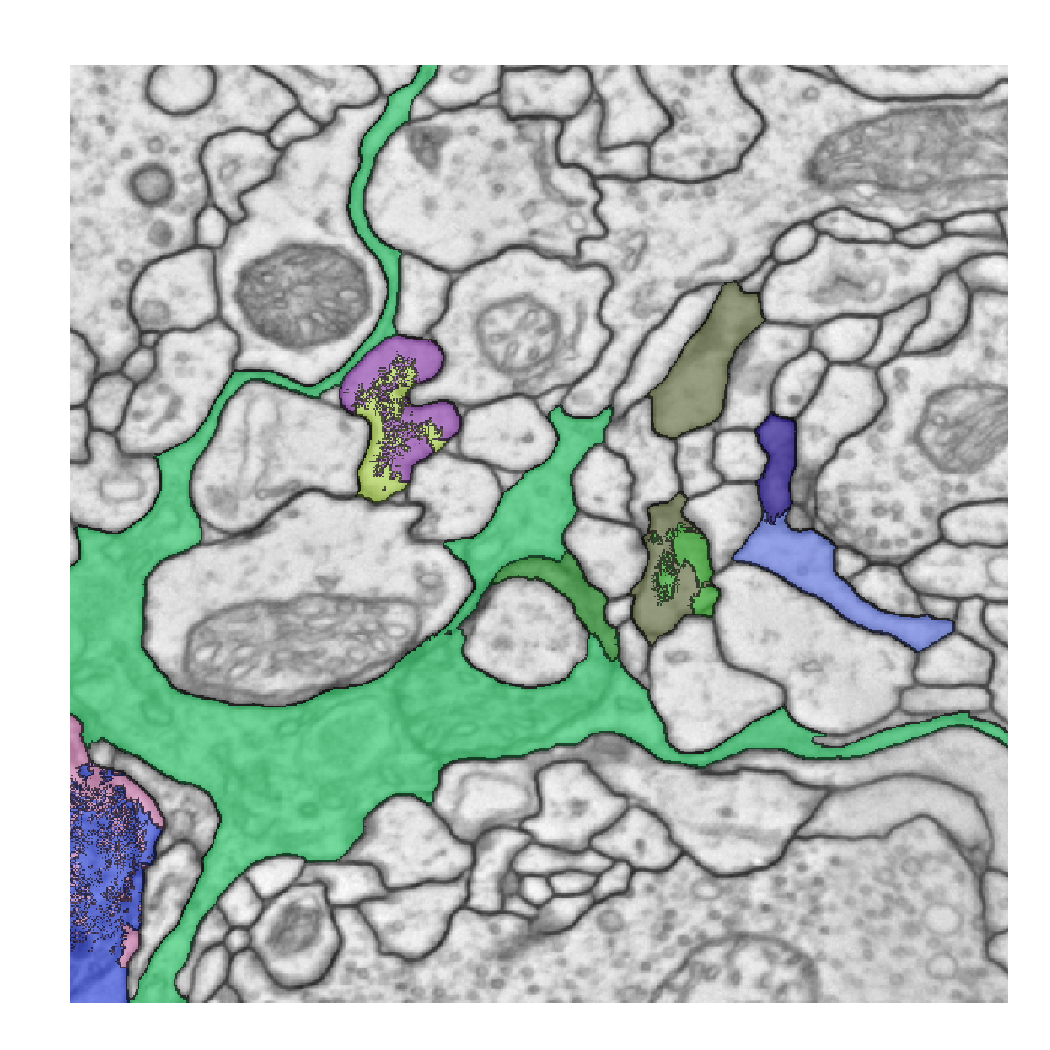
\includegraphics[width=0.98\textwidth]{figs/comparison/max_T.pdf}
%         % \caption{Watershed, seeded at local minima of the smoothed input map~(WS)} \label{fig:ws}
%     \end{subfigure}\hspace{0.5cm}%

% \begin{subfigure}[t]{0.46 \linewidth}
%         \centering
%         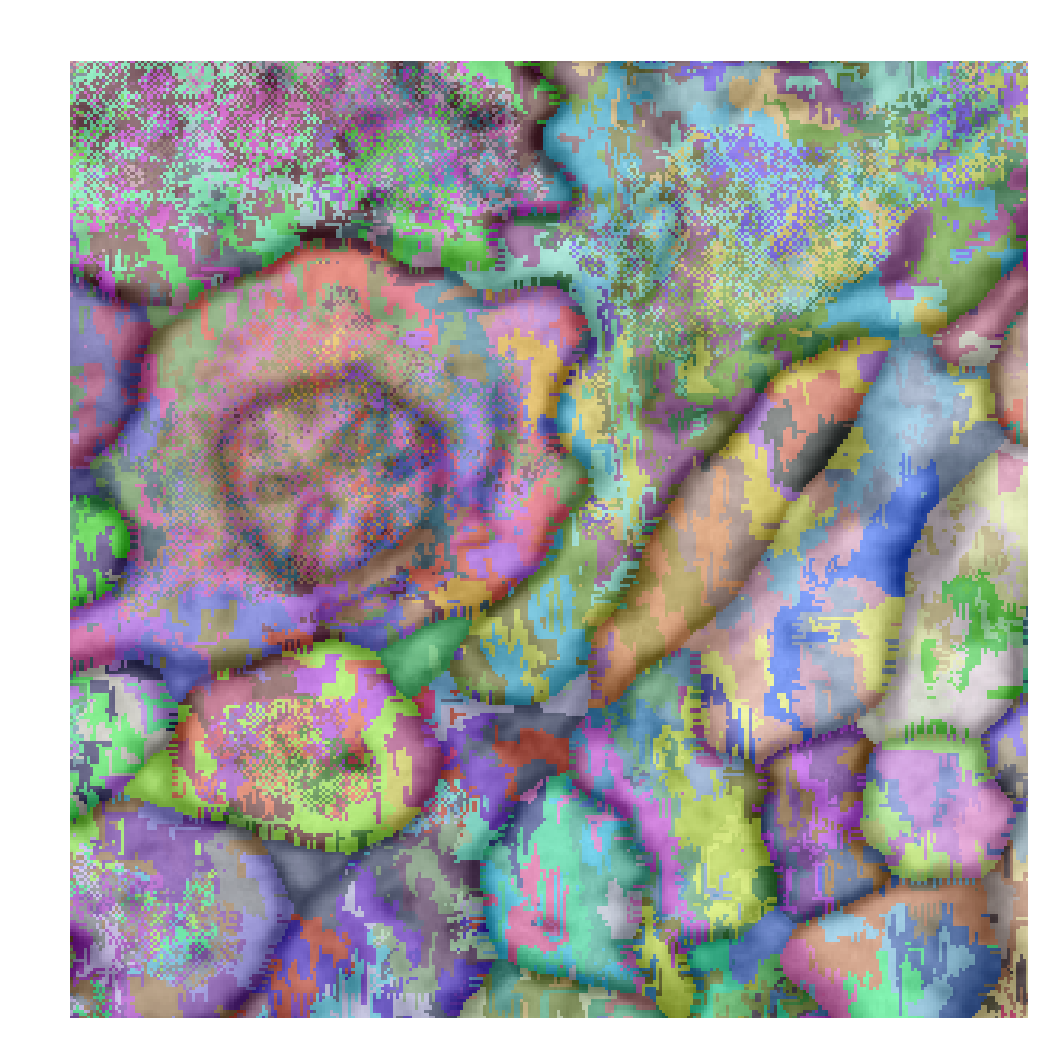
\includegraphics[width=0.98\textwidth]{figs/comparison/min_F.pdf}
%         % \caption{Thresholding of local boundary maps ~(THRESH)} \label{fig:thresh}
%     \end{subfigure}%
%     \begin{subfigure}[t]{0.46 \linewidth}
%         \centering
%         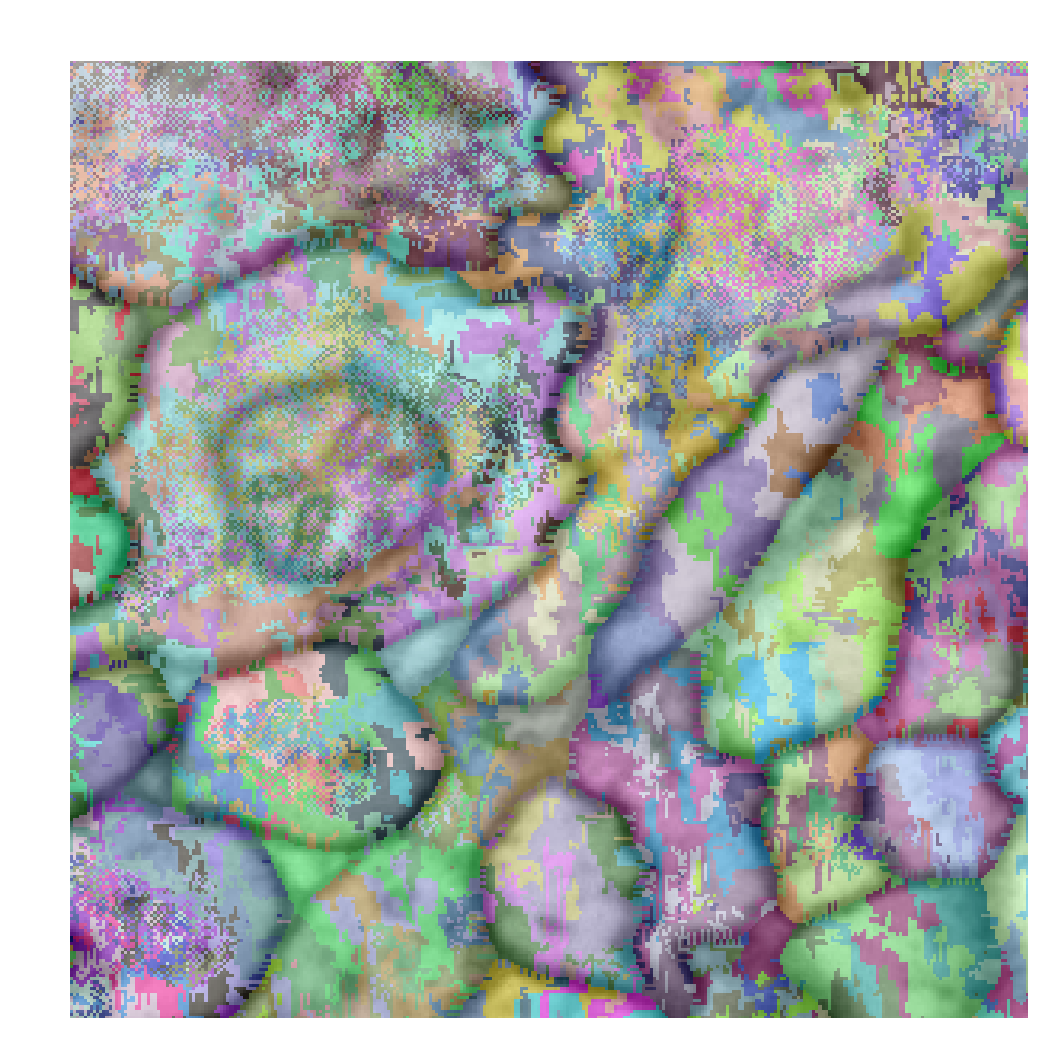
\includegraphics[width=0.98\textwidth]{figs/comparison/min_T.pdf}
%         % \caption{Watershed, seeded at local minima of the smoothed input map~(WS)} \label{fig:ws}
%     \end{subfigure}\hspace{0.5cm}%

%     % \vspace{-0.4cm}
%     \caption{Comparison of results from different update rules on signed graph with and without cannot-link constraints \TODO{add arrows/circles highlighting merge/split mistakes and correct decisions. Align; add captions}}
%     \label{fig:isbi-examples}
% \end{figure}% \captionsetup[


\subsection{Comparison of update rules} \label{sec:exp_first_comparison}
\begin{itemize}
  \item Highlight difference of the sum in Fig. \ref{fig:intro_figure}
  \item compare different choices of signed-cost-mappings (say which one worked best)
  \item present cremi crop-C table and rule out single and complete linkage
\end{itemize}




